%%!TEX TS-program = latex
\documentclass[12pt,letterpaper]{article}
\usepackage{epsfig}                 
\usepackage[authoryear]{natbib}
\usepackage{graphicx}
\usepackage{amsmath}
\usepackage{psfrag}
\usepackage{mathabx}
\renewcommand{\baselinestretch}{1.6}
\large
\pagenumbering{arabic}
\usepackage[usenames,dvipsnames]{color}
\usepackage{fullpage}
\bibliographystyle{genetics}
\usepackage{multirow}
\newcommand{\ye}{\hat{y}}
\newcommand{\xe}{\hat{x}}
\usepackage{color}
\usepackage[normalem]{ulem}  

\title{Sperm modifiers of female drive.}
\author{Yaniv Brandvain \\ email: ybrandvain@gmail.com  \and Graham Coop \\ email: gmcoop@ucdavis.edu }

\usepackage{fancyhdr}
\pagestyle{fancy}
\lhead{}
\rhead{}
\renewcommand{\headrulewidth}{0.0pt}
\rfoot{}
\cfoot{\thepage}
\date{}
\bibliographystyle{plain}
\begin{document}
\maketitle
\begin{center}
Center for Population Biology \& Department of Evolution and Ecology \\ University of California - Davis \\ Davis, CA, 95616
\end{center}

%FIgures 
{\bf Abstract:}
\newpage

\section*{Introduction}

%Since all alleles within an individual rely on individual survival and reproduction for evolutionary success, most of life in a diploid eukaryotic genome is harmonious.
%However, this harmony is incomplete, as in numerous cases an allele can benefit (in the short or long term) from taking advantage of its host.
Despite the apparent unity of the organism, occasionally alleles can
gain an evolutionary advantage at a cost to  individual fitness
\citep{Burt2006}, often by exploiting meiosis and gametogensis.
%A clear opportunity for this conflict arises during gametogenesis where alternative alleles are in direct competition for representation in the next generation.
Female meiosis, an asymmetric event in which only one of two alternate alleles
enters the  egg, with the others consigned to the polar body, is one such occasion \citep{Sandler1957,Pardo-ManuelDeVillena2001a}. 
%Female meiosis is particularly unfair, only one of the four products of meiosis becomes an egg, while the other threes are disgarded into polar bodies. 
An allele that biases female meiosis in its favor (i.e. a meiotic driver), may increase in frequency even if this driver entails a pleiotropic fitness cost \citep{Prout1973}, generating a genetic conflict between the success of the driver and organismal fitness.
%Alleles that can segregate into the egg more than half the time in heterozygotes, by exploiting asymmetries, 
%can potentially increase in frequency in the population (i.e. experiencing true meiotic drive).
%If such alleles have fitness consequences they are a source of genetic conflict, 
%and can become balanced in the population if their host in homozygotes 
%out weighs their ability to spread to spread through heterozygotes. 
Meiotic drivers observed in nature (in both plants
\citep{Buckler1999,Fishman2005,Fishman2008}, and animals
\citep{Agulnik1990,Wu2005,Pardo-ManuelDeVillena2001c}) highlight this
conflict -- the selfish benefits of drive and the associated
pleiotropic fitness costs sustain a balanced polymorphism
\citep{Prout1973}, 
and often generate on ongoing evolutionary escalation of drive suppressors and enhancers \citep{Dawe1996,Fishman2008}. 
%Such balanced drive systems can cause the subsequent evolution of linked enhancers of drive
%and of supressors of drive throughout the genome. 
%Indeed, the known polymorphic female meiotic drive systems (OM, maize knobs, IN, mimulus, others?) habor
%a great diversity of enhancers and supressors. 
The threat of meiotic drive to organismal fitness is potentially so
severe that it has been hypothesized that many basic properties of meiosis and o\"{o}genesis, including the initial genome doubling in meiosis I \citep{Haig1991}, the commonness of arrested female meiosis \citep{Mira1998}, and sex differences in the recombination rate \citep{Haig2010,Brandvain2012} have evolved to disrupt meiotic drive and enforce fairness.

It is therefore somewhat surprising that despite the intense evolutionary pressure on female meiosis to prevent meiotic drive, 
it is potentially open to sabotage by a virtual stranger -- a haploid sperm genome.
That is, in many animal species, the completion of female meiosis requires fertilization of the egg, 
and there is ample opportunity for interaction between the sperm and female meiotic machinery.
If, for example, an allele in sperm could facilitate meiotic drive by a genetically equivalent allele in a 
heteromorphic dyad, such an allele could presumably bias meiosis in its favor and rapidly spread through the population.
At first sight, it seems as although female meiosis is primed to be exploited by selfish sperm systems.  

%Another unusual aspect of animal female meiosis is the fact that it is paused at XXX.
%In fact in many species of animal the final stages of female meiosis are only completed upon fertlization of the egg by sperm.There's considerable variation in 
%which stage of meiosis requires fertilization.
%This raises the possibility that an allele in sperm could influence the outcome of meiosis in its favor. 
%For example imagine an allele that when a sperm bearing this allele were to encounter an egg, whose meiotic product was currently heterozygote for 
%another copy of itself, the sperm allele biased meiosis in favor of the other copy of itself.
%At first sight, it seems as although female meiosis is primed to be exploited by selfish sperm systems. 

Why then is the requirement of fertilization to complete female meiosis so ubiquitous? 
It is certainly not the case that animals are mechanistically incapable of evolving past this requirement.
There is considerable variation in which stage of meiosis requires fertilization, and 
a number of animal clades (should we try and lower bound how many transitions?) have evolved
to allow the completion of female meiosis upon ovulation. 
%(Although even in these organisms female meiosis 
%may also be subjection to influence by sperm alleles, if the sperm arrives at the egg soon enough after 
%ovulation to influence meiosis.) 

It is also not the case that sperm is mechanistically incapable of influencing the outcome of female meiosis.
%This is not just idle speculation, as there is also direct evidence that sperm components and indeed different sperm genotypes can affect female meiosis.
%are mechanistic reasons to think that this is more than idle speculation.
Mechanistic evidence for this possibility comes from \emph{C. elegans}, where experimentally suppressing XXX leads to premature deployment of the aster (a vital component of mitotic machinery) provided by the sperm, disrupting MII meiotic segregation in the egg, leading to a triploid zygote. 
%This demonstrates that physical components derived from the sperm are are capable of affecting the outcome of female meiosis.
Additionally, genetic evidence suggests that the transmission patterns in heterozygous females can depend on sperm haplotype. 
Specifically, the two best characterized female meiotic drive systems in mouse (In and Om), both operate by distorting the second meiotic division, 
and in both systems the outcome of female meiosis depends the genotype of the fertilizing sperm \citep{Agulnik1993,Wu2005}. 


In this article we explore through simple population genetic models the consequences of alleles that influence the outcome 
of female meiosis. 
We use these models to argue that it is actually surprisingly hard for the influence of
sperm on the outcome of meiosis to drive sustained conflict. In fact we find that sperm and egg 
genomes' interests are often aligned as they are both invested in the fate of the zygote they will form (as was suggested for the In locus \citep{Pomiankowski1993}).
This suggests that females are unlikely to evolve to prevent the influence of sperm on meiosis,
and indeed features of meiosis may evolve that facilitate the interaction of sperm with female meiosis. 

\section*{Results}

\yb{YB: To me its (1) male enhancement of female drive cannot maintain a stable polymorphisms, and (2) An allele in sperm can evolve to suppress its drive in females.}


Rough order of rest of text
\subsection*{A single locus model} 
The standard model of female meiotic drive is two allele model, where the
allele $1$ is transmitted $d$ fraction of the time through female
meiosis ($d > \half$), regardless of the genotype of the sperm. 
In mammals, fertilization takes place at MII, so we imagine this drive must be taking place at MII in order
for a sperm to have any influence. For drive to take place at MII there has to be an uneven number of
 crossovers between the centromere and the drive locus, such that realistically $d$ is bounded to be $<0.75$?. 
In other systems where fertilization occurs during MI, sperm could influence either drive at MI or MII, 
and drivers at MI can have a $d=1$ if they occur in tight linkage with the centromere.

We can model a simple sperm dependent meiotic drive system, by
modifying this model so that the allele only drives during female
meiosis if it fertilized by a sperm carrying that allele
 (see
Figure \ref{Eggsperm_2_allele_cartoon}). Under what conditions can
this self propograting driver allele spread, and could it drive the
evolution of supressors? 

We first consider the situation where the driving allele has no
fitness consequences in heterozygotes, only in homozygotes (whose
relative fitness is $1-s$). A standard meiotic drive allele can always
invade the population in this situation, as it is initially only
present mostly in heterozygotes and rarely suffers the consequences of
the problems in homozygotes. However, if the cost in homozygotes is
strong enough ($s>XXd$), then the allele is prevented from reaching
fixation and instead is maintained as a balanced polymorphism in the
population \citep{Prout1973}. Such balanced polymorphisms can then
drive the evolution of supressors of drive \citep{XX}, and most of our
examples of drive systems are of this form. 

Under a recessive fitness cost model our sperm dependent driver
actually has far more restrictive conditions to invade the population,
than a standard meiotic driver (see Figure \ref{Invasion_space}).
That is because our allele which drives only when it is present in the
fertilizing sperm is guarenteed to form a homzygote. Thus, 
to even spread in the population when it is rare, our sperm-dependent
driver has to overcome the cost it suffers in the homozygote state.

When conditions are suitable for such alleles to spread into the
population, they spread slowly through low frequencies as they rarely
drive as they are unlikely to be fertilized by a sperm with the right
allele. Once they become established they spread rapidly due to their
positive frequency dependent behavior (Inset in Figure \ref{Invasion_space}). 
Unlike standard meiotic drive systems 
these alleles can not become balanced in the population  by homozygote
cost, as they have already over come this cost just to enter the population.


HETERO

\begin{figure}
	\rotatebox{270}{\includegraphics[width = 0.8
          \textwidth]{Figures/sperm_egg_cartoon1.ps}}
\caption{transmission probabilities for alleles through female
  meiosis depend on sperm genotype. 2 allele model}  
\label{Eggsperm_2_allele_cartoon}
\end{figure}

\begin{figure}
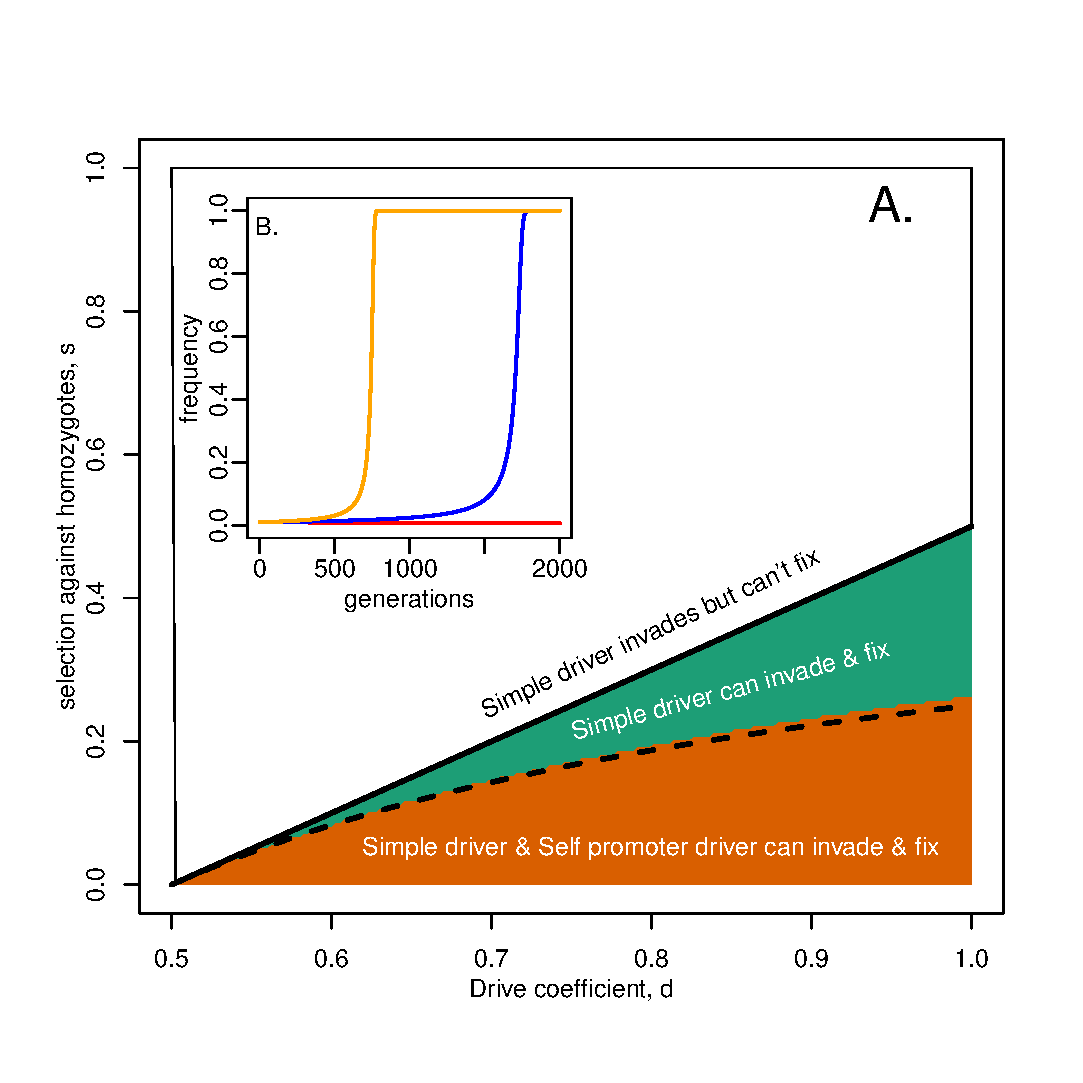
\includegraphics[width = 0.8 \textwidth]{Figures/invasion_space_recessive_driver.eps}
\caption{Invasion analysis. Likely merge with Figure 1.} \label{Invasion_space}
\end{figure}





Cost of alleles

We'll setup a model where the sperm allele affects outcome of female meiosis. This may not be biologically
realistic as there is very little sperm expression. More realistically the male genotype that produced the sperm
may be more relevant, as males could place products in their sperm that influenced the outcome of female meoisis.
However, in practice models that allow the influence of fertilizing male genotype on female meiosis 
seem to behave very similiarly to those based on the allele of the fertilizing sperm.
For simplicity we'll focus on models based on the allele of the sperm, as it's bloodly complicated enough already.

\subsection*{ A) Invasion by single self promoting allele}




show that such alleles:
\begin{enumerate}
\item can't be balanced, \\
\item and homozygous problems are tested out at low freq.  \\
\item Any heterozygous problems, leads to a bistable allele\\
\item If these alleles take off they speed through to fixation\\
\item If allele has any drive ability in absence of sperm effect that is what allows it to enter the population
and sperm effect isn't a further cause of conflict. What if anything do we mean by this?\\
\item PERHAPS HERE WE INTRODUCE A SELF-RESTRAINING ALLELE
\end{enumerate}

Conclusion, such alleles are unlikely to cause evolution of female supressors, they test hemselves in a homozygous
state when they enter the population, and sweep quickly (all the way to fixation) if they enter the pop at all.\\

\begin{figure}
	\rotatebox{270}{\includegraphics[width = 0.8
          \textwidth]{Figures/sperm_egg_cartoon2.ps}}
\caption{transmission probabilities righthand allele through female
  meiosis}  \label{Eggsperm_3_allele_cartoon}
\end{figure}


\subsection*{B) A more biologically realistic selfish sperm system}
Three allele systems. See Figure \ref{Eggsperm_3_allele_cartoon} \\ 
Perhaps these self promoting alleles are biologically unrealistic as new alleles needs 
both ability to drive in female meiosis and to influence that drive in sperm.
Perhaps more realistic to think that a female drive system evolves, 
and then a sperm modifier appears. This will only occur if original system is trapped 
at drive-selection balance. So driver must have homozygous cost.

\begin{enumerate}
\item Setup a drive-selection balanced polymorphism in std. drive model. 
Do this by imagining the sperm-influence allele arising on the background of the driver, 
so the allele has drive capabilities, and can have had time to evolve new biology. 
Evolving on the new background means that the allele suffers the fitness consequences of the 
driver.  See A in Figure \ref{Eggsperm_3_allele_cartoon} \\
\item Sperm-based enhancers of drive can't invade (can they in some situations?). \\
\item Intuition is that the driver has already driven to a frequency 
where it is held in check by its cost in homozygotes. The sperm allele 
thus can't really help as it creates zygotes which suffer the homozygous fitness consequences.
\end{enumerate}

\subsection{So what can evolve?}
So what can happen?
\begin{enumerate}
\item Alleles that arise in linkage with drive systems, which when in sperm switch off drive, 
can spread. They benefit from drive, but avoid some of the
consequences ( (Bi) in Figure \ref{Eggsperm_3_allele_cartoon} ). Overall as a side product they are benefiting all in pop.\\
\item Presumably alleles that actually switch the allele that drives may do even better? As they'd end up in 
hets. Although they'd not drive, so hard to say. YB: There is evidence that In distorts meiosis in the other direction (they still drive when rare i.e. when not fused with drive supp sperm) \\
\item Alleles that cause sperm to switch off drive that arise on other background or unlinked to the drive system
are selected, and spread as fast as female supressors of drive ( (Bii) in Figure \ref{Eggsperm_3_allele_cartoon} )..\\
\item Alleles that in females facilitate the action of sperm supressors of drive (or vis versa) can spread. Haven't actually checked this.\\
\end{enumerate}

\section*{Conclusions.}
Discussion of general conclusion that females have little reason to evolve supression mechanisms to prevent sperm influence on meiosis. 
General logic that sperm genome has to live in a zygote with consequences of its effect on female meiosis, so
it can not generate too dire a consequence.
I THINK THERE IS A MORE SUBTLE POINT . The sperm has special knowledge that if it allows drive it will end up in the low fitness homozygote. 


This logic may not hold for sex chromosomes. In ZW systems 
 Male modification of recombination rates
POssibility that this could happen in plants if pollen emit signals to ``egg''
Discussion of OM and IN.

\bibliography{refs}
\end{document}


